\section{Interactivité}
\label{s:interactivité}

Il y a deux modes d'interaction avec l'application: le clavier et la souris.
Le clavier est utilisé pour entrer des raccourcis permettant d'effectuer des actions alors que la souris permet de contrôler les éléments de l'interface graphique.

\subsection{Raccourcis clavier}
Les raccourcis clavier disponible sont les suivants:

\begin{table}[h]
    \begin{center}
    \begin{tabular}{|c|l|}
        \hline
        \multicolumn{1}{|c|}{Touche} & \multicolumn{1}{c|}{Action}\\
        \hline
        ctrl+Z / ctrl+Y & \emph{Undo} / \emph{Redo}\\
        Espace & Capture d'écran\\  
        Flèches gauche/droite & Rotation de la caméra autour de son axe Y local\\
        Flèches haut/bas & Rotation de la caméra autour de son axe X local\\
        A/D & Déplacement de la caméra sur son axe X local\\
        W/S & Déplacement de la caméra sur son axe Y local\\
        +/- & Déplacement de la caméra sur son axe Z local\\
        R & Réinitialisation de la pose de la caméra\\
        C & Changer le mode de projection de la caméra\\
        H & Afficher/cacher l'interface graphique\\
        1 & Créer une sphère\\
        2 & Créer un cube\\
        3 & Créer une ligne\\
        4 & Créer un triangle\\
        5 & Créer un rectangle\\
        6 & Créer un pentagone\\
        7 & Créer un cercle\\
        8 & Créer une flèche\\
        9 & Créer une étoile\\
        0 & Créer un mur en relief\\
        M & Créer un modèle 3D du Faucon Millenium\\
        X & Créer un modèle 3D d'un X-Wing Fighter\\
        P & Créer les deux portails\\
        B & Créer une courbe de Bézier\\
        N & Créer une courbe de Hermite\\
        E & Changer l'effet pleine fenêtre \\
        \hline
    \end{tabular}
    \caption{Raccourcis claviers de l'application}
    \end{center}
\end{table}
Il est à noter que les touches \emph{CTRL} droite et gauche fonctionnent pour les actions \emph{Undo} et \emph{Redo}.
De plus, le contrôle de la caméra s'effectue toujours dans son repère local.\\

\subsection{Interface graphique}
L'interface graphique comporte quatre panneaux.
Le premier est appelé \emph{Scène} et il se situe en haut à gauche de l'écran (voir figure \ref{fig:scene}).
Il affiche la liste des \emph{GameObjects} présents dans la scène.
Au démarrage de l'application, seule la lumière est présente, mais la liste se met à jour à chaque fois qu'on nouvel élément est ajouté à la scène.
Les objets sont affichés dans la liste dans l'ordre qu'ils sont créés et leur ordre n'est pas modifiable.
Il est possible de sélectionner un \emph{GameObjects} en cliquant sur le petit bouton à gauche de son nom dans la liste, ce qui modifie les autres panneaux de l'interface en conséquence.\\

\begin{figure}[H]
    \centering
	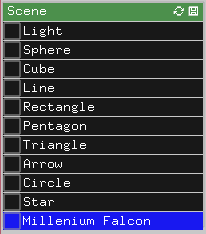
\includegraphics[scale=0.7]{fig/scene.png}
	\caption{Scène}
	\label{fig:scene}
\end{figure}

Le second panneau est appelé \emph{Inspecteur} et se situe à droite de l'écran (voir figure \ref{fig:inspecteur}).
Il permet de modifier les attributs du \emph{GameObject} présentement sélectionné.
Les attributs modifiables dans l'inspecteur dépendent du type de \emph{GameObject} qui est sélectionné.
Les différentes sections du chapitre sur les fonctionnalités présenteront quels attributs sont modifiables pour chaque type d'objet.\\

\begin{figure}[H]
    \centering
	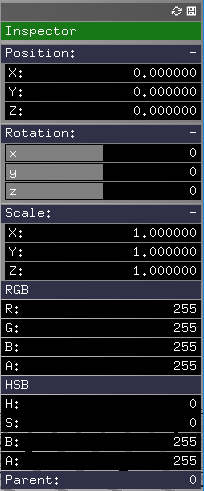
\includegraphics[scale=0.55]{fig/inspecteur.png}
	\caption{Inspecteur}
	\label{fig:inspecteur}
\end{figure}

Le troisième panneau de contrôle est celui des textures (voir figure \ref{fig:texture}).
Il s'affiche en bas à gauche de l'écran uniquement lorsqu'un \emph{GameObject} 2D (ligne, rectangle, triangle, cercle ou pentagone) est sélectionné.
Ce panneau permet de choisir la texture de l'objet 2D parmi les 5 textures procédurales offertes.

\begin{figure}[H]
    \centering
	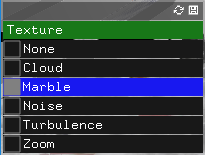
\includegraphics[scale=0.6]{fig/texture.png}
	\caption{Texture}
	\label{fig:texture}
\end{figure}

Le dernier panneau présent dans l'interface graphique est celui du mode d'éclairage (voir figure \ref{fig:mode_eclairage}).
Il s'affiche en bas à gauche de l'écran uniquement lorsque la lumière est sélectionnée.
Ce panneau permet de choisir parmi un des quatre types de lumière classiques, soient ponctuel, directionnel, projecteur et ambiant.

\begin{figure}[H]
    \centering
	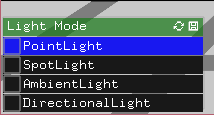
\includegraphics[scale=0.8]{fig/lightmode.png}
	\caption{Mode d'éclairage}
	\label{fig:mode_eclairage}
\end{figure}

Enfin, la seule sortie de l'application est une capture d'écran qu'il est possible d'effectuer en appuyant sur la barre espace (voir section \ref{ss:capture_ecran}).
\clearpage
